\section{Experiments}\label{sec:experiments}

We test the scaling laws from Sections~4--5 and translate them into actionable configuration strategies when a key parameter varies across CIFAR-100 with ResNet-18. Experiment sets are run: optimal performance of different optimizers and their corresponding learning rates (Exp.~1), $\eta$--$\lambda$ interaction (Exp.~2), $B$, $\lambda$, and $\eta$ coupling (Exp.~3), and $B$, $\lambda$, and $\eta$ coupling in LLM fine-tuning (Exp.~4).

% \begin{tcolorbox}
% \textbf{Q3:} In practical scenarios, when a key parameter varies, how can this law be translated into actionable configuration strategies to guide the adaptive adjustment of the remaining parameters?
% \end{tcolorbox}

\subsection{Setup}
For detailed experimental setup and evaluation methods, please refer to the Appendix \ref{Appendix:exp}.

\begin{figure*}[t]
    \centering
    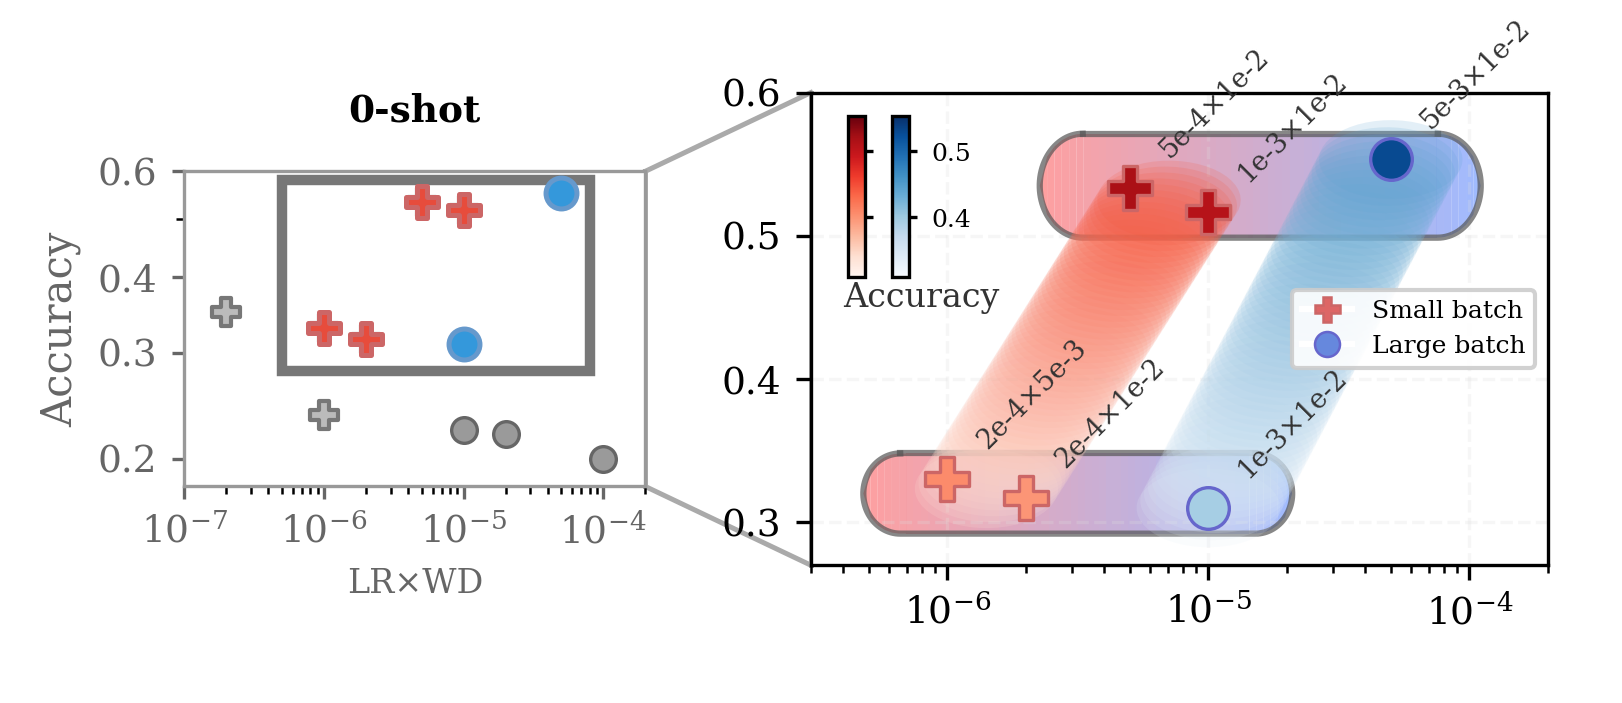
\includegraphics[width=\linewidth]{figures/LLM (1).png}
    \vspace{-.6cm}
    \caption{Coupled effects of the batch size $B$ and optimization hyperparameters (learning rate $\eta$ and weight decay $\lambda$) in training Qwen3-0.6B. We consider a small batch size ($B=32$) and a large batch size ($B=128$), and evaluate performance on SVAMP.}
    \label{fig:LLM1}
    \vspace{-1em}  
\end{figure*}


\subsection{Results}

\paragraph{Exp.\ 1: Optimal performance and corresponding LR.}
The theory (Theorems \ref{thm:sgd-WD}, \ref{thm:sgdm-WD}) predicts better generalization and stricter learning rate bounds as we add weight decay, hence $\varepsilon_{\text{SGD}} > \varepsilon_{\text{SGD+WD}}$, $\varepsilon_{\text{SGDM}} > \varepsilon_{\text{SGDM+WD}}$ and $\eta^*_{\text{SGD}} > \eta^*_{\text{SGD+WD}}$, $\eta^*_{\text{SGDM}} > \eta^*_{\text{SGDM+WD}}$. Figure~\ref{fig:performance} confirms this ordering: Introducing $\lambda$ leads to smaller generalization error and optimal learning rates for both SGD+WD and SGDM+WD. Table~\ref{tab:exp1} (in Appendix \ref{Appendix:exp}) summarizes the best configurations from our search. Plain SGD peaks at $\eta^* \approx 0.3$ ($73.61\%$ test accuracy). 
Adding momentum ($\beta{=}0.1$) without WD as a new baseline SGDM yields $\eta^* \approx 0.15$ ($73.47\%$). With WD $\lambda{=}0.005$, SGD+WD attains $\eta^* \approx 0.25$ and $78.29\%$; SGDM+WD with $\lambda{=}0.0015$ reaches $\eta^* \approx 0.1$ and $78.61\%$. WD clearly improves generalization but requires a commensurate reduction in $\eta$ to stay within the stable regime.
%In practice, when adding $\lambda$, $\eta$ should be reduced to retain optimal generalization.


\begin{table}[t]
\caption{Optimal accuracy and corresponding LR by optimizer.}
\label{tab:exp1}
\vspace{-0.5em}
\centering
\small
\begin{tabular}{lcc}
\toprule
Optimizer & $\eta^*$ & Test acc. (\%) \\
\midrule
SGD & 0.30 & 73.61 \\
SGD+WD ($\lambda{=}0.005$) & 0.25 & 78.29 \\
SGDM ($\beta{=}0.1$, no WD) & 0.15 & 73.47 \\
SGDM+WD ($\beta{=}0.8$, $\lambda{=}0.0015$) & 0.10 & 78.61 \\
\bottomrule
\end{tabular}
\vspace{-0.5em}
\end{table}



\paragraph{Exp.\ 2: $\eta$--$\lambda$ interaction.}
With momentum $0.9$ and batch size $128$ fixed, we check the inverse scaling $\lambda =\mathcal{O}( 1/\eta)$ (Eq.~\ref{coupling:lamda}). 
For fixed $T$, Eq.~\eqref{coupling:lamda} implies that high accuracy should lie along a trade-off where larger $\eta$ pairs with smaller $\lambda$. 
Figure~\ref{fig:WD and LR}(a) shows test accuracy over $\eta \in [0.01, 0.3]$ and $\lambda \in [10^{-5}, 10^{-2}]$. 
The high-accuracy region forms a band consistent with $\eta \cdot \lambda \approx \text{const}$: from high-$\eta$/low-$\lambda$ (e.g.\ $\eta{=}0.2$, $\lambda{=}5{\times}10^{-4}$) to low-$\eta$/high-$\lambda$ (e.g.\ $\eta{=}0.05$, $\lambda{=}5{\times}10^{-3}$). 
Increasing $\eta$ while keeping performance requires proportionally decreasing $\lambda$, and vice versa. 
Keeping $\eta \cdot \lambda$ in a moderate range preserves test performance when varying either parameter.
To make this scaling law directly visible without diagonal heatmap reading, we additionally replot each fixed-$\lambda$ curve against the joint product $\eta\times\lambda$ (Fig.~\ref{fig:WD and LR}(b,c)): all curves attain both their lowest train loss and highest test accuracy inside the same narrow $\eta\times\lambda$ band, providing a quantitative one-dimensional confirmation of Eq.~\eqref{coupling:lamda}.

\paragraph{Exp.\ 3: $B$, $\lambda$, and $\eta$ coupling.}
We test the batch-size coupling (Eq.~\ref{coupling:Batch}) using the linear rule $\eta \propto B$ and $B \in \{32, 128, 256, 512\}$. 
Eq.~\eqref{coupling:Batch} predicts that $B$ is positively coupled with $\eta$ and $\lambda$; under linear LR scaling $\eta \propto B$, optimal $\lambda$ should increase with $B$. 
Figure~\ref{fig:batch} demonstrates that the optimal $\lambda$ and effective $\eta \cdot \lambda$ grow with batch size. When scaling batch size, both learning rate and weight decay should be scaled up (e.g., linear LR rule and proportionally larger $\lambda$) to preserve generalization.
For instance, the green location shifts indicate that best $\lambda$ at $B{=}32$ shifts to higher values at $B{=}128$.

\paragraph{Robustness across architectures and random seeds.}
To verify that the three predictions above do not rely on a single architecture or a single random initialization, we additionally rerun Exp.~1--3 on \textbf{VGG-16} (no residual connections, $14.8$M params) and \textbf{ResNet-50} ($23.5$M params), each with two random seeds (42, 123); ResNet-18 is independently rerun four times (two seeds $\times$ two runs each). 
This adds up to roughly $640$ training runs in total, all reported as mean $\pm$ half-range. 
We summarise the cross-architecture findings here and defer per-architecture tables, full heatmaps, and stability summaries to Appendix~\ref{Appendix:robustness}.
(i) The stability boundary ordering $\eta^{*}_{\text{SGD+WD}}>\eta^{*}_{\text{SGD}}>\eta^{*}_{\text{SGDM+WD}}$ is unanimous across all three architectures; SGD and SGDM+WD always peak at $\eta^{*}=0.1$, while SGD+WD peaks on a broad plateau $\eta^{*}\in[0.5,1.0]$. 
(ii) The anti-diagonal $\eta$--$\lambda$ pattern of Exp.~2 is preserved on every architecture; at $\eta=0.2$, all eight independent runs (R18$\times$4 + VGG$\times$2 + R50$\times$2) unanimously select $\lambda^{*}=5\!\times\!10^{-4}$. 
(iii) Under the linear LR rule of Exp.~3, the optimal $\lambda^{*}$ stays in $[5\!\times\!10^{-4},\,10^{-3}]$ for all four batch sizes on every architecture. 
Half-ranges are below $0.5\%$ in the stable region and only grow near the divergence boundary, confirming that the conclusions are seed- and architecture-robust.

\paragraph{Exp.\ 4: Coupling among $B$, $\lambda$, and $\eta$ in LLM fine-tuning.}
We examine whether the $\eta$–$\lambda$ trade-off observed in Exp.~2 persists in a realistic LLM fine-tuning regime. Concretely, we fine-tune Qwen3-0.6B with LoRA on MathInstruct and evaluate out-of-distribution generalization on SVAMP. We sweep the learning rate $\eta$ and weight decay $\lambda$ over a log-spaced grid, while holding the LoRA configuration (e.g., rank) and the optimization schedule fixed (constant learning rate, no warmup). Performance is measured by exact-match accuracy of the final SVAMP answer under a fixed prompting template and decoding protocol, which are kept identical across all hyperparameter settings for a controlled comparison. We report results under 0-shot prompting.

%As shown in Fig.~\ref{fig:LLM1}, 8-shot prompting underperforms 0-shot across a broad region of the $(\eta,\lambda)$ grid. One plausible explanation is that adding in-context exemplars substantially increases the effective prompt length and compositional complexity, thereby worsening position-related degradation: the actual query and its key constraints are pushed toward later positions in the sequence, where attention and conditioning can be weaker, leading the model to rely more on superficial template cues than on the problem-specific details required for an exact final answer.

In language modeling experiments based on Qwen3-0.6B, we similarly validate the hyperparameter scaling law after incorporating batch size. As illustrated in the Figure \ref{fig:LLM1}, for a fixed performance level, the blue points (corresponding to larger batch sizes) consistently lie to the right of the red points (corresponding to smaller batch sizes). Since the horizontal axis represents increasing joint values of $\eta\times\lambda$ (from $10^{-6}$ to $10^{-4}$), this indicates that larger batch sizes require larger joint values to achieve the same performance. These results further confirm, at a larger scale, that maintaining stability at comparable performance levels necessitates that the batch size scales proportionally with $\eta\times\lambda$. 